% Options for packages loaded elsewhere
\PassOptionsToPackage{unicode}{hyperref}
\PassOptionsToPackage{hyphens}{url}
%
\documentclass[
]{article}
\usepackage{lmodern}
\usepackage{amssymb,amsmath}
\usepackage{ifxetex,ifluatex}
\ifnum 0\ifxetex 1\fi\ifluatex 1\fi=0 % if pdftex
  \usepackage[T1]{fontenc}
  \usepackage[utf8]{inputenc}
  \usepackage{textcomp} % provide euro and other symbols
\else % if luatex or xetex
  \usepackage{unicode-math}
  \defaultfontfeatures{Scale=MatchLowercase}
  \defaultfontfeatures[\rmfamily]{Ligatures=TeX,Scale=1}
\fi
% Use upquote if available, for straight quotes in verbatim environments
\IfFileExists{upquote.sty}{\usepackage{upquote}}{}
\IfFileExists{microtype.sty}{% use microtype if available
  \usepackage[]{microtype}
  \UseMicrotypeSet[protrusion]{basicmath} % disable protrusion for tt fonts
}{}
\makeatletter
\@ifundefined{KOMAClassName}{% if non-KOMA class
  \IfFileExists{parskip.sty}{%
    \usepackage{parskip}
  }{% else
    \setlength{\parindent}{0pt}
    \setlength{\parskip}{6pt plus 2pt minus 1pt}}
}{% if KOMA class
  \KOMAoptions{parskip=half}}
\makeatother
\usepackage{xcolor}
\IfFileExists{xurl.sty}{\usepackage{xurl}}{} % add URL line breaks if available
\IfFileExists{bookmark.sty}{\usepackage{bookmark}}{\usepackage{hyperref}}
\hypersetup{
  pdftitle={LeastSquares},
  hidelinks,
  pdfcreator={LaTeX via pandoc}}
\urlstyle{same} % disable monospaced font for URLs
\usepackage[margin=1in]{geometry}
\usepackage{longtable,booktabs}
% Correct order of tables after \paragraph or \subparagraph
\usepackage{etoolbox}
\makeatletter
\patchcmd\longtable{\par}{\if@noskipsec\mbox{}\fi\par}{}{}
\makeatother
% Allow footnotes in longtable head/foot
\IfFileExists{footnotehyper.sty}{\usepackage{footnotehyper}}{\usepackage{footnote}}
\makesavenoteenv{longtable}
\usepackage{graphicx,grffile}
\makeatletter
\def\maxwidth{\ifdim\Gin@nat@width>\linewidth\linewidth\else\Gin@nat@width\fi}
\def\maxheight{\ifdim\Gin@nat@height>\textheight\textheight\else\Gin@nat@height\fi}
\makeatother
% Scale images if necessary, so that they will not overflow the page
% margins by default, and it is still possible to overwrite the defaults
% using explicit options in \includegraphics[width, height, ...]{}
\setkeys{Gin}{width=\maxwidth,height=\maxheight,keepaspectratio}
% Set default figure placement to htbp
\makeatletter
\def\fps@figure{htbp}
\makeatother
\setlength{\emergencystretch}{3em} % prevent overfull lines
\providecommand{\tightlist}{%
  \setlength{\itemsep}{0pt}\setlength{\parskip}{0pt}}
\setcounter{secnumdepth}{-\maxdimen} % remove section numbering

\title{LeastSquares}
\author{}
\date{\vspace{-2.5em}}

\begin{document}
\maketitle

\hypertarget{introduction}{%
\section{1. Introduction}\label{introduction}}

The \color{blue}
\href{https://www.archive.ics.uci.edu/ml/datasets/Bike+Sharing+Dataset}{dataset}
\color{black} for this project is the ``Bike Sharing Dataset Data Set''
found in the UCI Machine Learning Repository. The dataset contains
hourly count of rental bikes for all of 2011 and 2012 (January 1, 2011
to December 31, 2012) in the Capital Bikeshare System of Washington D.C.
area (Washington-Arlington-Alexandria, DC-VA-MD-WV metropolitan area).
The UCI Machine Learning Repository cites Hadi Fanaee-T from the
``Laboratory of Artificial Intelligence and Decision Support (LIAAD),
University of Porto'' for the compilation of the data.

The dataset is outdated since data is actually available up to November
2020 on Capital Bikeshare's website (as of December 18, 2020), but this
limited dataset will still work for the purposes of demonstrating linear
algebra on a real world dataset.

There are 14 different variables that are in this dataset that are
potentially of interest. Two variables are not useful and immediately
thrown out: \texttt{instant} (this is simply the row number of the
dataset) and \texttt{dteday} (date of the year).

Denote \(x_{n}\) as plausible independent variables and denote \(y_{n}\)
as plausible dependent variables.

\(x_{1}\): \texttt{season} (1: spring, 2: summer, 3: fall, 4: winter)

\(x_{2}\): \texttt{yr} (0: 2011, 1: 2012)

\(x_{3}\): \texttt{mnth} (1 to 12)

\(x_{4}\): \texttt{hour} (0 to 23)

\(x_{5}\): \texttt{holiday} (whether a holiday (0 or 1) from
\color{blue}
\href{https://dchrc.dc.gov/page/holiday-schedule}{this list of holidays}
\color{black} )

\(x_{6}\): \texttt{weekday} (0 to 6)

\(x_{7}\): \texttt{workingday} (1 if weekday and not holiday, 0
otherwise)

\(x_{8}\): \texttt{temp} (0-1, normalized temperature in Celsius.
Divided by 41)

\(x_{9}\): \texttt{atemp} (0-1, normalized ``feels like'' temperature in
Celsius. Divided by 50)

\(x_{10}\): \texttt{hum} (percent humidity)

\(x_{11}\): \texttt{windspeed} (0-1, Normalized wind speed. Divided by
67)

\(y_{1}\): \texttt{casual} (count of casual users)

\(y_{2}\): \texttt{registered} (count of registered users)

\(y_{3}\): \texttt{cnt} (count of sum of casual and registered users)

The following least squares regression exercise will try to predict the
\texttt{casual}, \texttt{registered}, or \texttt{cnt} as a function of
the independent variables.

\hypertarget{data-analysis}{%
\subsection{Data Analysis}\label{data-analysis}}

Preliminary data analysis shows that the \texttt{hour} is by far the
most important independent variable for explaining the variation in the
dependent variables. Thus, it is important to know how exactly the
\texttt{hour} variable interacts with \texttt{registered},
\texttt{casual}, and \texttt{cnt}.

Although there are three different dependent variables,

It could sense to treat \texttt{hour} as a categorical variable (treat
\texttt{hour} as 23 independent variables, one for each hour minus the
constant term), but in this case, we will try to fit \texttt{hour} in
terms of a polynomial curve.

\begin{figure}
\centering
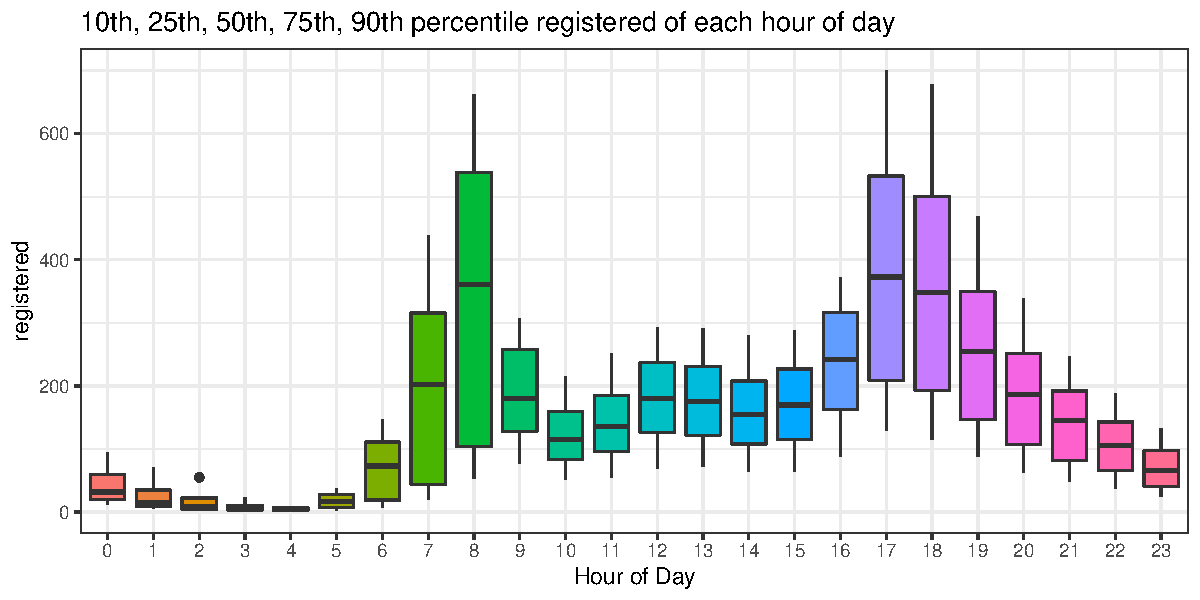
\includegraphics{LeastSquares_files/figure-latex/unnamed-chunk-1-1.pdf}
\caption{Boxplot of registered users for Jan 1, 2011 to December 31,
2011 for each hour of day. The low whisker represents 10th percentile,
the box represents the interquartile range, the top whisker represents
the 90th percentile}
\end{figure}

\begin{figure}
\centering
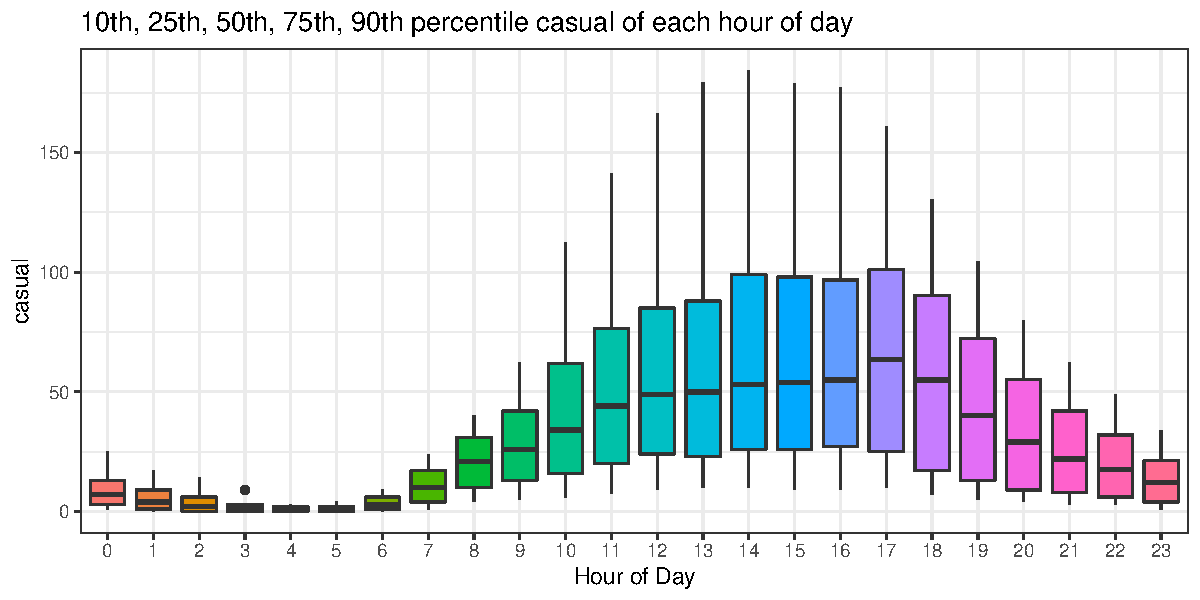
\includegraphics{LeastSquares_files/figure-latex/unnamed-chunk-2-1.pdf}
\caption{Boxplot of casual users for Jan 1, 2011 to December 31, 2011
for each hour of day. The low whisker represents 10th percentile, the
box represents the interquartile range, the top whisker represents the
90th percentile}
\end{figure}

\begin{figure}
\centering
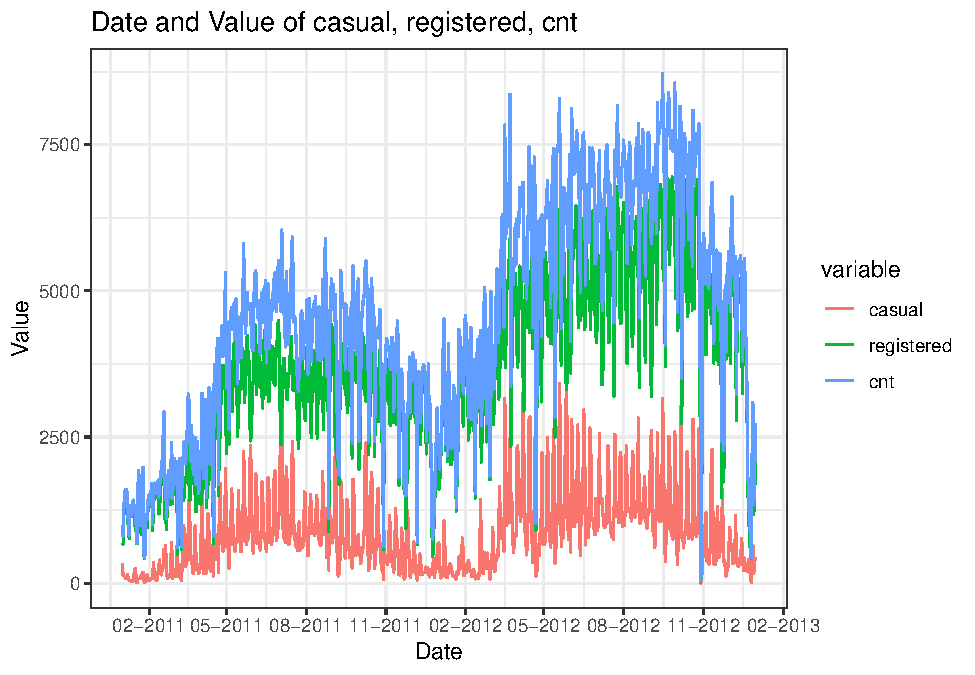
\includegraphics{LeastSquares_files/figure-latex/unnamed-chunk-3-1.pdf}
\caption{Number of casual, registered, and sum of casual and registered
for all 731 days in the dataset}
\end{figure}

\begin{figure}
\centering
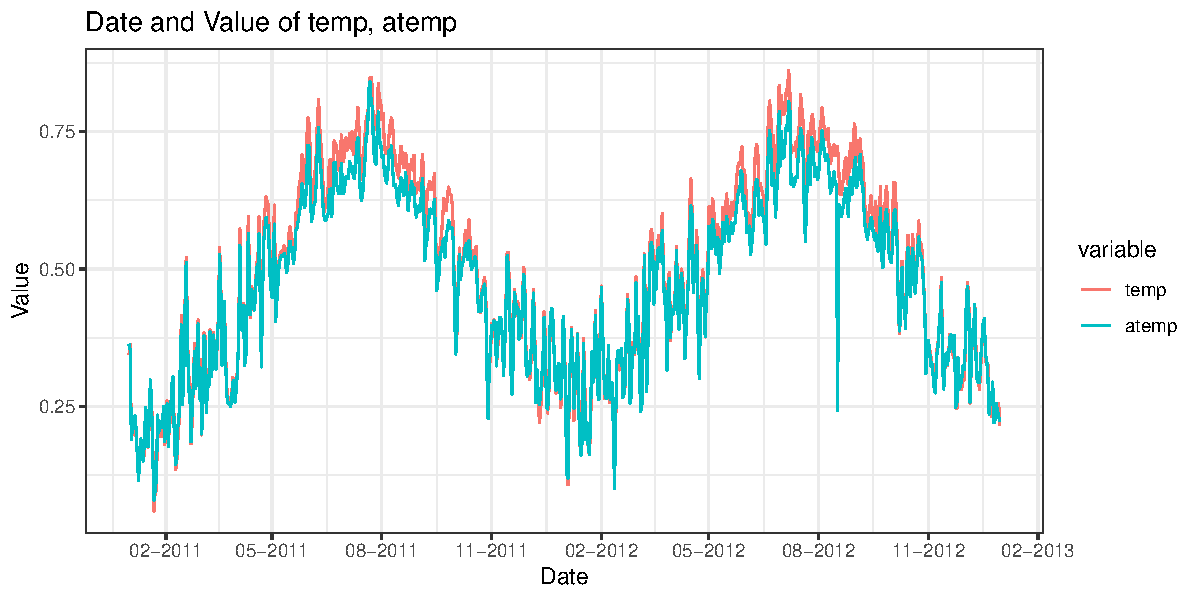
\includegraphics{LeastSquares_files/figure-latex/unnamed-chunk-4-1.pdf}
\caption{Normalized temperature and ``feels like'' temperature for all
731 days in the datset}
\end{figure}

\newpage

\hypertarget{design-matrix}{%
\section{2. Design Matrix}\label{design-matrix}}

\begin{longtable}[]{@{}lrrr@{}}
\caption{R-squared values of y}\tabularnewline
\toprule
& \(R^{2}_{cnt}\) & \(R^{2}_{casual}\) &
\(R^{2}_{registered}\)\tabularnewline
\midrule
\endfirsthead
\toprule
& \(R^{2}_{cnt}\) & \(R^{2}_{casual}\) &
\(R^{2}_{registered}\)\tabularnewline
\midrule
\endhead
\(h\) & 0.343 & 0.285 & 0.291\tabularnewline
\(h+h^{2}\) & 0.464 & 0.371 & 0.394\tabularnewline
\(h+h^{2}+h^{3}\) & 0.515 & 0.430 & 0.431\tabularnewline
\(h+h^{2}+\dots+h^{4}\) & 0.516 & 0.440 & 0.436\tabularnewline
\(h+h^{2}+\dots+h^{5}\) & 0.530 & 0.446 & 0.464\tabularnewline
\(h+h^{2}+\dots+h^{6}\) & 0.552 & 0.446 & 0.497\tabularnewline
\(h+h^{2}+\dots+h^{7}\) & 0.589 & 0.446 & 0.551\tabularnewline
\(h+h^{2}+\dots+h^{8}\) & 0.599 & 0.446 & 0.565\tabularnewline
\(h+h^{2}+\dots+h^{9}\) & 0.606 & 0.447 & 0.575\tabularnewline
\(h+h^{2}+\dots+h^{10}\) & 0.606 & 0.447 & 0.575\tabularnewline
\(h+h^{2}+\dots+h^{11}\) & 0.613 & 0.447 & 0.585\tabularnewline
\(h+h^{2}+\dots+h^{12}\) & 0.614 & 0.447 & 0.585\tabularnewline
\(h+h^{2}+\dots+h^{13}\) & 0.638 & 0.448 & 0.619\tabularnewline
\(h+h^{2}+\dots+h^{14}\) & 0.638 & 0.448 & 0.619\tabularnewline
\(h+h^{2}+\dots+h^{15}\) & 0.638 & 0.448 & 0.619\tabularnewline
\bottomrule
\end{longtable}

\begin{longtable}[]{@{}lrrrrrrr@{}}
\toprule
expr & min & lq & mean & median & uq & max & neval\tabularnewline
\midrule
\endhead
design\_matrix() & 19.831 & 20.682 & 23.796 & 21.782 & 24.580 & 57.546 &
100\tabularnewline
design\_matrix\_Cpp() & 8.825 & 9.160 & 10.775 & 9.532 & 10.675 & 22.519
& 100\tabularnewline
mode.matrix.lm() & 19.763 & 20.907 & 26.939 & 22.960 & 28.242 & 184.484
& 100\tabularnewline
\bottomrule
\end{longtable}

\hypertarget{normal-equation}{%
\section{3. Normal Equation}\label{normal-equation}}

\begin{longtable}[]{@{}llll@{}}
\toprule
\begin{minipage}[b]{0.17\columnwidth}\raggedright
\strut
\end{minipage} & \begin{minipage}[b]{0.16\columnwidth}\raggedright
\(\kappa(A)\)\strut
\end{minipage} & \begin{minipage}[b]{0.16\columnwidth}\raggedright
\(\kappa(A)^{2}\)\strut
\end{minipage} & \begin{minipage}[b]{0.40\columnwidth}\raggedright
Relative error/error message\strut
\end{minipage}\tabularnewline
\midrule
\endhead
\begin{minipage}[t]{0.17\columnwidth}\raggedright
\(h\)\strut
\end{minipage} & \begin{minipage}[t]{0.16\columnwidth}\raggedright
\(8.05 \times 10^{1}\)\strut
\end{minipage} & \begin{minipage}[t]{0.16\columnwidth}\raggedright
\(6.49 \times 10^{3}\)\strut
\end{minipage} & \begin{minipage}[t]{0.40\columnwidth}\raggedright
\(5.87 \times 10^{-12}\)\strut
\end{minipage}\tabularnewline
\begin{minipage}[t]{0.17\columnwidth}\raggedright
\(h+h^{2}\)\strut
\end{minipage} & \begin{minipage}[t]{0.16\columnwidth}\raggedright
\(1.45 \times 10^{3}\)\strut
\end{minipage} & \begin{minipage}[t]{0.16\columnwidth}\raggedright
\(2.09 \times 10^{6}\)\strut
\end{minipage} & \begin{minipage}[t]{0.40\columnwidth}\raggedright
\(-1.1 \times 10^{-14}\)\strut
\end{minipage}\tabularnewline
\begin{minipage}[t]{0.17\columnwidth}\raggedright
\(h+h^{2}+h^{3}\)\strut
\end{minipage} & \begin{minipage}[t]{0.16\columnwidth}\raggedright
\(3.01 \times 10^{4}\)\strut
\end{minipage} & \begin{minipage}[t]{0.16\columnwidth}\raggedright
\(9.08 \times 10^{8}\)\strut
\end{minipage} & \begin{minipage}[t]{0.40\columnwidth}\raggedright
\(1.18 \times 10^{-12}\)\strut
\end{minipage}\tabularnewline
\begin{minipage}[t]{0.17\columnwidth}\raggedright
\(h+h^{2}+\dots+h^{4}\)\strut
\end{minipage} & \begin{minipage}[t]{0.16\columnwidth}\raggedright
\(6.46 \times 10^{5}\)\strut
\end{minipage} & \begin{minipage}[t]{0.16\columnwidth}\raggedright
\(4.17 \times 10^{11}\)\strut
\end{minipage} & \begin{minipage}[t]{0.40\columnwidth}\raggedright
\(2.87 \times 10^{-12}\)\strut
\end{minipage}\tabularnewline
\begin{minipage}[t]{0.17\columnwidth}\raggedright
\(h+h^{2}+\dots+h^{5}\)\strut
\end{minipage} & \begin{minipage}[t]{0.16\columnwidth}\raggedright
\(1.42 \times 10^{7}\)\strut
\end{minipage} & \begin{minipage}[t]{0.16\columnwidth}\raggedright
\(2.03 \times 10^{14}\)\strut
\end{minipage} & \begin{minipage}[t]{0.40\columnwidth}\raggedright
\(1.52 \times 10^{-8}\)\strut
\end{minipage}\tabularnewline
\begin{minipage}[t]{0.17\columnwidth}\raggedright
\(h+h^{2}+\dots+h^{6}\)\strut
\end{minipage} & \begin{minipage}[t]{0.16\columnwidth}\raggedright
\(3.59 \times 10^{8}\)\strut
\end{minipage} & \begin{minipage}[t]{0.16\columnwidth}\raggedright
\(1.29 \times 10^{17}\)\strut
\end{minipage} & \begin{minipage}[t]{0.40\columnwidth}\raggedright
Error, Recripocal \(\kappa(A)\): \(5.89 \times 10^{-18}\)\strut
\end{minipage}\tabularnewline
\begin{minipage}[t]{0.17\columnwidth}\raggedright
\(h+h^{2}+\dots+h^{7}\)\strut
\end{minipage} & \begin{minipage}[t]{0.16\columnwidth}\raggedright
\(1.06 \times 10^{10}\)\strut
\end{minipage} & \begin{minipage}[t]{0.16\columnwidth}\raggedright
\(1.12 \times 10^{20}\)\strut
\end{minipage} & \begin{minipage}[t]{0.40\columnwidth}\raggedright
Error, Recripocal \(\kappa(A)\): \(6.14 \times 10^{-21}\)\strut
\end{minipage}\tabularnewline
\begin{minipage}[t]{0.17\columnwidth}\raggedright
\(h+h^{2}+\dots+h^{8}\)\strut
\end{minipage} & \begin{minipage}[t]{0.16\columnwidth}\raggedright
\(3.33 \times 10^{11}\)\strut
\end{minipage} & \begin{minipage}[t]{0.16\columnwidth}\raggedright
\(1.11 \times 10^{23}\)\strut
\end{minipage} & \begin{minipage}[t]{0.40\columnwidth}\raggedright
Error, Recripocal \(\kappa(A)\): \(6.35 \times 10^{-24}\)\strut
\end{minipage}\tabularnewline
\begin{minipage}[t]{0.17\columnwidth}\raggedright
\(h+h^{2}+\dots+h^{9}\)\strut
\end{minipage} & \begin{minipage}[t]{0.16\columnwidth}\raggedright
\(1.10 \times 10^{13}\)\strut
\end{minipage} & \begin{minipage}[t]{0.16\columnwidth}\raggedright
\(1.22 \times 10^{26}\)\strut
\end{minipage} & \begin{minipage}[t]{0.40\columnwidth}\raggedright
Error, Recripocal \(\kappa(A)\): \(6.78 \times 10^{-27}\)\strut
\end{minipage}\tabularnewline
\begin{minipage}[t]{0.17\columnwidth}\raggedright
\(h+h^{2}+\dots+h^{10}\)\strut
\end{minipage} & \begin{minipage}[t]{0.16\columnwidth}\raggedright
\(3.82 \times 10^{14}\)\strut
\end{minipage} & \begin{minipage}[t]{0.16\columnwidth}\raggedright
\(1.46 \times 10^{29}\)\strut
\end{minipage} & \begin{minipage}[t]{0.40\columnwidth}\raggedright
Error, Recripocal \(\kappa(A)\): \(1.29 \times 10^{-29}\)\strut
\end{minipage}\tabularnewline
\begin{minipage}[t]{0.17\columnwidth}\raggedright
\(h+h^{2}+\dots+h^{11}\)\strut
\end{minipage} & \begin{minipage}[t]{0.16\columnwidth}\raggedright
\(1.39 \times 10^{16}\)\strut
\end{minipage} & \begin{minipage}[t]{0.16\columnwidth}\raggedright
\(1.94 \times 10^{32}\)\strut
\end{minipage} & \begin{minipage}[t]{0.40\columnwidth}\raggedright
Error, Recripocal \(\kappa(A)\): \(1.07 \times 10^{-32}\)\strut
\end{minipage}\tabularnewline
\begin{minipage}[t]{0.17\columnwidth}\raggedright
\(h+h^{2}+\dots+h^{12}\)\strut
\end{minipage} & \begin{minipage}[t]{0.16\columnwidth}\raggedright
\(5.38 \times 10^{17}\)\strut
\end{minipage} & \begin{minipage}[t]{0.16\columnwidth}\raggedright
\(2.89 \times 10^{35}\)\strut
\end{minipage} & \begin{minipage}[t]{0.40\columnwidth}\raggedright
Error, Recripocal \(\kappa(A)\): \(7.16 \times 10^{-35}\)\strut
\end{minipage}\tabularnewline
\begin{minipage}[t]{0.17\columnwidth}\raggedright
\(h+h^{2}+\dots+h^{13}\)\strut
\end{minipage} & \begin{minipage}[t]{0.16\columnwidth}\raggedright
\(2.21 \times 10^{19}\)\strut
\end{minipage} & \begin{minipage}[t]{0.16\columnwidth}\raggedright
\(4.86 \times 10^{38}\)\strut
\end{minipage} & \begin{minipage}[t]{0.40\columnwidth}\raggedright
Error, Recripocal \(\kappa(A)\): \(1.13 \times 10^{-37}\)\strut
\end{minipage}\tabularnewline
\begin{minipage}[t]{0.17\columnwidth}\raggedright
\(h+h^{2}+\dots+h^{14}\)\strut
\end{minipage} & \begin{minipage}[t]{0.16\columnwidth}\raggedright
\(5.86 \times 10^{22}\)\strut
\end{minipage} & \begin{minipage}[t]{0.16\columnwidth}\raggedright
\(3.43 \times 10^{45}\)\strut
\end{minipage} & \begin{minipage}[t]{0.40\columnwidth}\raggedright
Error, Recripocal \(\kappa(A)\): \(2.67 \times 10^{-40}\)\strut
\end{minipage}\tabularnewline
\begin{minipage}[t]{0.17\columnwidth}\raggedright
\(h+h^{2}+\dots+h^{15}\)\strut
\end{minipage} & \begin{minipage}[t]{0.16\columnwidth}\raggedright
\(4.51 \times 10^{22}\)\strut
\end{minipage} & \begin{minipage}[t]{0.16\columnwidth}\raggedright
\(2.04 \times 10^{45}\)\strut
\end{minipage} & \begin{minipage}[t]{0.40\columnwidth}\raggedright
Error, Recripocal \(\kappa(A)\): \(2.51 \times 10^{-43}\)\strut
\end{minipage}\tabularnewline
\bottomrule
\end{longtable}

\begin{longtable}[]{@{}lrrrrrrr@{}}
\toprule
expr & min & lq & mean & median & uq & max & neval\tabularnewline
\midrule
\endhead
normal\_equations(A, b) & 6.045 & 6.601 & 9.521 & 7.551 & 9.587 & 78.223
& 100\tabularnewline
normal\_equations\_Cpp(A, b) & 4.806 & 5.100 & 6.516 & 5.872 & 7.349 &
13.222 & 100\tabularnewline
\bottomrule
\end{longtable}

\hypertarget{qr-decomposition}{%
\section{4. QR Decomposition}\label{qr-decomposition}}

\begin{longtable}[]{@{}lrrrrrrr@{}}
\toprule
expr & min & lq & mean & median & uq & max & neval\tabularnewline
\midrule
\endhead
qr.solve(A, b) & 5.315 & 5.743 & 8.441 & 6.576 & 8.769 & 23.07 &
100\tabularnewline
qr\_solve\_Cpp(A, b) & 5.277 & 5.629 & 6.554 & 6.176 & 6.970 & 10.95 &
100\tabularnewline
\bottomrule
\end{longtable}

\hypertarget{singular-value-decomposition}{%
\section{5. Singular Value
Decomposition}\label{singular-value-decomposition}}

\begin{longtable}[]{@{}lrrrrrrr@{}}
\toprule
expr & min & lq & mean & median & uq & max & neval\tabularnewline
\midrule
\endhead
svd\_solve(A, b) & 9.591 & 10.415 & 13.097 & 11.413 & 14.236 & 26.682 &
100\tabularnewline
svd\_solve\_Cpp(A, b) & 8.219 & 8.881 & 10.449 & 9.491 & 11.173 & 26.194
& 100\tabularnewline
\bottomrule
\end{longtable}

\begin{longtable}[]{@{}lrrrrrrr@{}}
\toprule
expr & min & lq & mean & median & uq & max & neval\tabularnewline
\midrule
\endhead
normal\_equations(A, b) & 5.999 & 6.281 & 7.377 & 6.588 & 7.369 & 15.332
& 100\tabularnewline
normal\_equations\_Cpp(A, b) & 4.791 & 4.983 & 5.500 & 5.305 & 5.702 &
8.665 & 100\tabularnewline
qr.solve(A, b) & 5.390 & 5.761 & 7.674 & 6.124 & 7.306 & 17.659 &
100\tabularnewline
qr\_solve\_Cpp(A, b) & 5.317 & 5.615 & 6.218 & 5.936 & 6.386 & 9.740 &
100\tabularnewline
svd\_solve(A, b) & 9.675 & 10.128 & 12.649 & 10.710 & 13.361 & 30.296 &
100\tabularnewline
svd\_solve\_Cpp(A,b) & 8.107 & 8.510 & 9.575 & 9.102 & 10.133 & 14.946 &
100\tabularnewline
\bottomrule
\end{longtable}

\begin{longtable}[]{@{}lrrrrrrr@{}}
\toprule
expr & min & lq & mean & median & uq & max & neval\tabularnewline
\midrule
\endhead
qr.solve(A, b) & 10.311 & 10.876 & 14.072 & 11.902 & 17.806 & 28.556 &
100\tabularnewline
qr\_solve\_Cpp(A, b) & 11.867 & 12.481 & 13.767 & 12.926 & 14.112 &
28.182 & 100\tabularnewline
svd\_solve(A, b) & 20.678 & 22.220 & 28.869 & 26.057 & 29.520 & 189.340
& 100\tabularnewline
svd\_solve\_Cpp(A,b) & 18.160 & 19.295 & 21.691 & 20.492 & 23.977 &
37.163 & 100\tabularnewline
\bottomrule
\end{longtable}

\hypertarget{final-regression-model}{%
\section{6. Final Regression Model}\label{final-regression-model}}

\(y_{1} = \beta_{0} + \beta_{1}x_{1} + \beta_{2}x_{2} + \beta_{3}x_{4} + \beta_{4}x_{4}^{2} + \beta_{4}x_{4}^{3} + \beta_{5}x_{9}\)

\(y_{3} = \beta_{0} + \beta_{1}x_{1} + \beta_{2}x_{2} + \beta_{3}x_{4} + \beta_{4}x_{4}^{2} + \beta_{5}x_{4}^{3} + \beta_{6}x_{4}^{4} + \beta_{7}x_{4}^{5} + \beta_{8}x_{4}^{6} + \beta_{9}x_{4}^{7} + \beta_{10}x_{8}\)

With the data inputted, we have

\(y_{1} = -42.145 + 0.6875x_{1} + 12.887x_{2} - 4.859x_{4} + 1.275x_{4}^{2} - 0.047x_{4}^{3} + 89.528x_{8}\)

\(y_{3} = -145.05 + 17.18x_{1} + 88.57x_{2} + 29.45x_{4} - 63.199x_{4}^{2} + 24.27x_{4}^{3} - 3.62x_{4}^{4} + 0.258x_{4}^{5} - 0.0088x_{4}^{6} + 0.000116x_{4}^{7} + 243.131x_{8}\)

Note that
\(\frac{1}{n}\sum_{i=1}^{n} x_{1} = \bar{x_{1}} = 2.50164, \frac{1}{n}\sum_{i=1}^{n} x_{2} = \bar{x_{2}} = 0.5025606, \frac{1}{n}\sum_{i=1}^{n} x_{8} = \bar{x_{8}} = 0.4970\).

\begin{verbatim}
## `summarise()` regrouping output by 'hr' (override with `.groups` argument)
## `summarise()` regrouping output by 'hr' (override with `.groups` argument)
\end{verbatim}

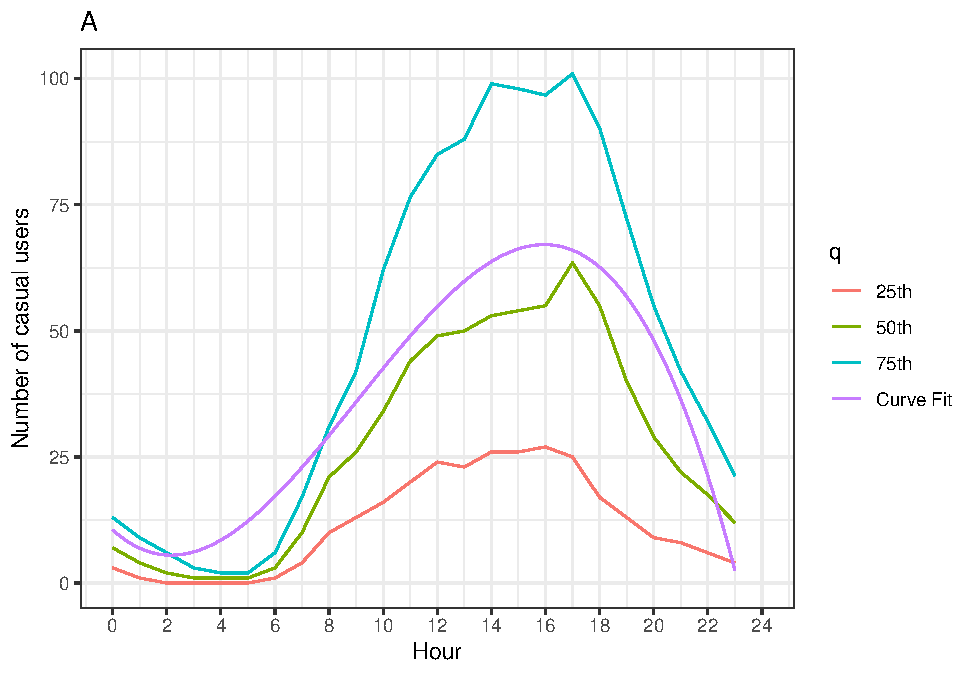
\includegraphics{LeastSquares_files/figure-latex/unnamed-chunk-14-1.pdf}
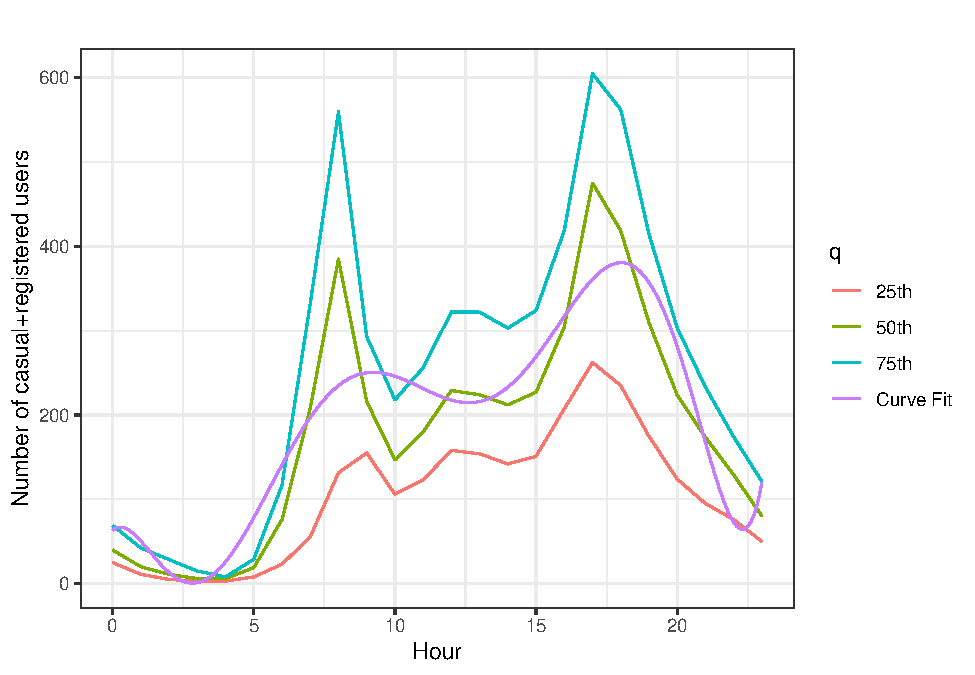
\includegraphics{LeastSquares_files/figure-latex/unnamed-chunk-14-2.pdf}

\end{document}
